% !TeX program = xelatex
% 混凝土骨料颗粒智能筛分比拼 — 评委阅读版（约20页目标）
% 编译: latexmk -xelatex main_submission.tex

\documentclass[UTF8,a4paper,11pt,fontset=fandol]{ctexart}

\usepackage[a4paper,top=2.05cm,bottom=2.05cm,left=2.15cm,right=2.15cm]{geometry}
\usepackage{graphicx}
\usepackage{xcolor}
\usepackage{booktabs}
\usepackage{amsmath,amssymb}
\usepackage{caption}
\usepackage{subcaption}
\usepackage{enumitem}
\usepackage{float}
\usepackage{hyperref}
\usepackage{tikz}
\usetikzlibrary{shapes,arrows,positioning}
\usepackage[numbers,sort&compress]{natbib}
\usepackage{array}
\usepackage[section]{placeins}

\captionsetup{font=footnotesize,labelfont=bf,width=0.94\linewidth,justification=raggedright,singlelinecheck=false}
\graphicspath{{figures/}{../../demo_data/samples/results/}{../../demo_data/samples/}{../assets/}}
\setlist{nosep,leftmargin=1.8em}
\setlength{\textfloatsep}{8pt plus 2pt minus 2pt}
\setlength{\floatsep}{7pt plus 2pt minus 2pt}
\setlength{\intextsep}{7pt plus 2pt minus 2pt}
\setlength{\abovedisplayskip}{6pt plus 2pt minus 2pt}
\setlength{\belowdisplayskip}{6pt plus 2pt minus 2pt}
\setlength{\emergencystretch}{8em}
\sloppy

\hypersetup{
  colorlinks=true,
  linkcolor=blue!55!black,
  citecolor=green!45!black,
  urlcolor=blue!65!black,
  pdftitle={混凝土骨料颗粒智能筛分技术报告：评委阅读版},
  pdfauthor={匿名},
  breaklinks=true
}

\title{\vspace{-1.2cm}\bfseries 混凝土骨料颗粒智能筛分技术报告\\[0.25em]
\large 自然堆积赛道：基于实例感知与质量级配映射的视觉筛分方法}
\author{}
\date{}

\begin{document}
\maketitle
\vspace{-1.5em}

\begin{abstract}
自然堆积场景下的骨料视觉筛分并不等价于“识别图像中的石子”。标准机械筛分以筛孔通过行为和逐级称重定义粒径级配，而单目图像直接获得的是二维可见轮廓及颗粒数量；因此，实例边界、像素尺度和统计口径之间存在连续的语义鸿沟。本文面向混凝土骨料颗粒智能筛分赛题，构建“实例感知--物理测量--筛分语义映射--任务输出”的分层方案：采用 ImageGrains 2.0 / Cellpose-SAM 预训练模型恢复颗粒实例，通过现场尺度标定获得毫米级长短轴、面积和形貌特征；进一步以短轴与等效直径构造可校准的筛分等效粒径，并用 $w=d^{\gamma}$ 将颗粒数量分布转换为质量相关分布，从而输出标准筛级质量占比及 $D_{10}/D_{50}/D_{90}$。同一实例几何还用于投影形貌分类和超限异常筛查。

当前三张自然堆积演示图像已形成从分割、几何测量到级配报告的完整闭环，共检测 3858 个实例。以 $\gamma=3$ 的未校准质量代理为例，三张图的数量型 $D_{50}$ 分别为 6.0、7.6 和 5.2~mm，而质量代理 $D_{50}$ 移动至 23.5、27.5 和 14.1~mm，说明从“按个数统计”到“按质量相关权重统计”会实质改变级配结论。仓库中的 27 项竞赛层合成测试已验证筛分映射、加权分位数、形貌、异常与报告逻辑的一致性；历史算法时序约为 27~s/张。需要强调的是，当前演示样本尚缺同批机械筛分逐筛称量真值，因此本文不将上述数值表述为筛分准确率。正式物理精度将通过“同批图像预测--机械筛分真值”配对实验校准并冻结 $\boldsymbol{\theta}$ 与 $\gamma$，再在独立批次上报告逐筛误差和 $D_p$ 误差。该方案的核心价值在于把预训练视觉能力与显式物理/统计校准结合，使最终输出既可自动化计算，也能追溯到颗粒实例与标准筛分语义。

\textbf{关键词：} 混凝土骨料；实例分割；Cellpose-SAM；粒径级配；机械筛分；质量加权
\end{abstract}

% ===== 1 问题定义与贡献 =====
\section{问题定义与主要贡献}
\label{sec:r-problem}

骨料粒径级配与颗粒形貌直接影响混凝土的堆积结构、工作性能和力学性能。工程检测通常依据 \texttt{GB/T 14685}、\texttt{JGJ 52} 等标准，通过逐级机械筛分和称重获得筛级质量占比及累计通过率\cite{gb14685-2022,jgj52-2006}。其物理意义明确，但取样、振筛、称量和记录均需要离线操作，难以直接嵌入生产过程形成快速反馈。本赛题因此要求参赛系统在自然堆积或输送场景中，以非人工筛分方式完成颗粒精细识别、粒径分析、形貌识别和异常检测，并在有限现场时间内给出可评价结果。

本任务与一般目标检测的根本区别在于：\textbf{比赛最终评价的是标准筛分语义，而不是图像中目标框或像素本身。} 从一幅自然堆积图像得到标准筛分级配，需要连续跨越三个层次。第一，自然堆积中的粘连、遮挡和阴影使“前景”必须进一步分解为独立颗粒；merge 会制造偏大的伪颗粒，split 会制造偏小实例。第二，像素轮廓必须通过本次成像条件的尺度标定转换为毫米量，否则长短轴和 50~mm 超限阈值没有物理意义。第三，也是最关键的一层，单目图像观察的是二维投影并天然按颗粒个数统计，而机械筛分反映三维颗粒的筛孔通过行为并按质量称重。因此，即使实例边界和毫米尺寸均准确，直接把二维短轴或数量分布当作机械筛分结果仍可能存在系统偏差。

图\ref{fig:r-three-gaps}把这三个问题组织为一条误差传播链。它们不是彼此独立的三个“功能点”：上游实例错误会改变几何量，几何量再经过质量幂次放大后影响场景级分位数。例如，两个相邻颗粒若被 merge 为一个实例，其短轴和面积通常增大；该伪粗颗粒又会在 $d^\gamma$ 权重下获得更大的质量贡献，因此最终偏差可能明显大于普通像素误差本身。相反，一个颗粒被 split 后会形成多个偏细实例，使数量统计和低粒径端同时增加。由此，本文不把实例分割精度、毫米尺度和级配映射分别优化后简单相加，而是始终围绕最终筛分语义检查误差如何向下游传播。

\begin{figure}[t]
\centering
\begin{tikzpicture}[
  node distance=0.55cm,
  stage/.style={rectangle,draw,rounded corners,minimum width=4.0cm,minimum height=1.0cm,align=center,font=\footnotesize},
  err/.style={rectangle,draw,dashed,rounded corners,minimum width=3.8cm,minimum height=0.85cm,align=center,font=\scriptsize},
  arr/.style={->,thick}
]
\node[stage,fill=blue!7] (s1) {图像 $I$ $\rightarrow$ 独立实例 $\{M_i\}$\\\textbf{鸿沟 1：接触/遮挡颗粒如何分离}};
\node[stage,fill=green!7,right=0.65cm of s1] (s2) {实例 $\{M_i\}$ $\rightarrow$ 毫米几何 $\mathbf{x}_i$\\\textbf{鸿沟 2：pixel 如何获得物理尺度}};
\node[stage,fill=orange!8,right=0.65cm of s2] (s3) {二维几何 $\rightarrow$ 标准筛分 $\mathcal{Y}$\\\textbf{鸿沟 3：投影/计数如何对应筛孔/称重}};
\node[err,below=0.55cm of s1] (e1) {merge：偏粗；split：偏细\\漏检/遮挡：代表性下降};
\node[err,below=0.55cm of s2] (e2) {尺度偏差近似按比例移动\\全部粒径和筛级边界};
\node[err,below=0.55cm of s3] (e3) {二维 $\neq$ 三维筛孔行为\\数量分布 $\neq$ 质量分布};
\draw[arr] (s1)--(s2); \draw[arr] (s2)--(s3);
\draw[arr] (s1)--(e1); \draw[arr] (s2)--(e2); \draw[arr] (s3)--(e3);
\end{tikzpicture}
\caption{自然堆积视觉筛分的三个连续语义鸿沟及其典型误差方向。系统设计的目标不是单独“做好分割”，而是控制这些误差向最终标准筛分结果的传播。}
\label{fig:r-three-gaps}
\end{figure}

据此，本文把任务形式化为一条分层测量链。给定图像 $I$，实例分割得到 $N$ 个可见颗粒掩膜
\begin{equation}
\mathcal{M}=\{M_i\}_{i=1}^{N}.
\end{equation}
对每个实例，经尺度恢复获得几何描述 $\mathbf{x}_i=(a_i,b_i,A_i,P_i,C_i,S_i,\ldots)$，其中 $a_i,b_i$ 为投影长短轴，$A_i,P_i$ 为面积与周长，$C_i,S_i$ 为圆度和凸度。随后构造筛分等效粒径 $d_i=f(\mathbf{x}_i;\boldsymbol{\theta})$、形貌类别 $c_i$ 和异常状态 $z_i$；再以质量代理权重 $w_i=d_i^{\gamma}$ 聚合为质量相关累计分布，输出 $D_{10}/D_{50}/D_{90}$ 与各标准筛级质量占比。完整链条可概括为
\begin{equation}
I\rightarrow\{M_i\}\rightarrow\{\mathbf{x}_i\}\rightarrow\{d_i,w_i\}\rightarrow\mathcal{Y}_{\mathrm{sieve}}.
\label{eq:r-pipeline}
\end{equation}

表\ref{tab:r-task-map}给出赛题任务与系统证据的直接对应关系。这里刻意把“输出”和“验证证据”分开：系统能够生成某类结果，只能证明功能存在；只有使用与该任务匹配的 ground truth，才能进一步声明准确率。

\begin{table}[t]
\centering
\caption{赛题任务、系统输出与最终验证证据。}
\label{tab:r-task-map}
\footnotesize
\renewcommand{\arraystretch}{1.12}
\begin{tabular}{>{\raggedright\arraybackslash}p{2.0cm}>{\raggedright\arraybackslash}p{5.2cm}>{\raggedright\arraybackslash}p{6.2cm}}
\toprule
任务 & 系统输出 & 最终应使用的验证证据 \\
\midrule
精细识别 & 独立实例 mask、实例数量、长短轴 & 人工实例掩膜；IoU/F1、merge/split \\
粒径分析 & $d_i$、$D_{10}/D_{50}/D_{90}$、逐筛级占比 & 同批机械筛分逐筛称量真值 \\
形貌分类 & AR、圆度、凸度及投影形貌类别 & 人工/专家二维形貌标签；三维针片状需物理量规 \\
异常检测 & $>50$~mm、过小和疑似泥团候选 & 已知异常目标或人工语义标签 \\
现场约束 & 标定、推理、质检与报告导出 & 完整 SOP wall-clock time \\
\bottomrule
\end{tabular}
\end{table}

围绕上述问题，本文的贡献集中在三点。其一，复用 ImageGrains 2.0\cite{mair2026imagegrains2} 与 Cellpose-SAM\cite{pachitariu2025cellposeSAM} 的预训练颗粒实例感知能力，降低比赛现场重新标注和训练的依赖，并把模型输出限制为可检查的实例轮廓与几何量。其二，不把二维短轴直接视为标准筛孔粒径，而是提出低维、可解释、可由机械筛分真值校准的“筛分等效粒径 + 质量加权”映射，将视觉数量统计转换到标准筛分关注的质量级配。其三，将粒径、投影形貌、异常筛查和现场操作组织为同一条可追溯数据链，同时明确区分功能演示、软件一致性和物理精度三种证据等级，避免把未配对机械筛分的视觉结果过度解释为准确率。

下一节说明为什么选择“强预训练视觉基座 + 显式物理/统计校准”，以及各模块如何组成在线推理链和离线校准环。

% ===== 2 总体框架 =====
\section{总体框架与技术路线}
\label{sec:r-framework}

技术路线的选择需要同时满足三项约束：能够分离自然堆积中的接触颗粒；尽量不依赖现场重新标注训练；最终输出必须能够与机械筛分真值建立明确映射。传统阈值/分水岭实现简单，但对背景、阴影和弱接触边界敏感；监督式实例分割可针对赛题训练，却需要代表性实例标注并承担现场域变化风险；多视角或深度方案能恢复更多三维信息，但设备、标定和现场布置复杂度更高。预训练颗粒实例模型则把最依赖大规模视觉数据的“边界识别”交给已有模型，同时允许赛题特有的毫米尺度和筛分口径通过少量物理数据显式校准。因此本文选择 ImageGrains 2.0 / Cellpose-SAM 作为上游基座，而不是从头训练一个端到端网络\cite{stringer2021cellpose,pachitariu2025cellposeSAM,mair2026imagegrains2}。

\begin{table}[t]
\centering
\caption{候选路线与本赛题约束的简化比较。}
\label{tab:r-route}
\footnotesize
\renewcommand{\arraystretch}{1.12}
\begin{tabular}{>{\raggedright\arraybackslash}p{3.1cm}>{\raggedright\arraybackslash}p{3.1cm}>{\raggedright\arraybackslash}p{3.0cm}>{\raggedright\arraybackslash}p{4.1cm}}
\toprule
路线 & 接触颗粒 & 数据/现场成本 & 本文判断 \\
\midrule
阈值/分水岭 & 强粘连易 merge/split & 低，但参数依赖场景 & 适合作为受控条件基线 \\
监督式实例分割 & 可学习复杂边界 & 实例标注和训练成本较高 & 有数据时可增强，但不作为现场依赖 \\
预训练颗粒实例模型 & 直接输出实例轮廓 & 可零样本部署 & 作为主感知基座 \\
多视角/深度/点云 & 可恢复部分第三维 & 标定、硬件和部署成本高 & 作为后续物理升级方向 \\
\bottomrule
\end{tabular}
\end{table}

本文系统采用“在线单向推理 + 离线物理校准”的结构，如图\ref{fig:r-architecture}。在线阶段从图像和尺度参考出发，依次得到实例掩膜、毫米级几何量、筛分等效粒径和质量级配；形貌与异常作为几何特征的并行分支，最终汇总为场景级报告。离线阶段使用与图像同批次的机械筛分结果拟合筛分映射参数 $\boldsymbol{\theta}$ 与质量指数 $\gamma$，校准完成后冻结参数，正式测试时不再根据测试结果临时调节。

\begin{figure}[t]
\centering
\begin{tikzpicture}[
  node distance=0.55cm and 0.42cm,
  block/.style={rectangle,draw,rounded corners,minimum height=0.85cm,minimum width=2.25cm,align=center,font=\footnotesize},
  small/.style={rectangle,draw,rounded corners,minimum height=0.68cm,minimum width=2.0cm,align=center,font=\scriptsize},
  arr/.style={->,thick}, fb/.style={->,thick,dashed}
]
\node[block,fill=blue!7] (img) {图像采集\\尺度参考};
\node[block,fill=blue!7,right=of img] (seg) {实例感知\\$I\to\{M_i\}$};
\node[block,fill=green!7,right=of seg] (geo) {物理测量\\$\{M_i\}\to\mathbf{x}_i$};
\node[block,fill=orange!8,right=of geo] (map) {筛分映射\\$d_i,w_i$};
\node[small,fill=orange!8,below=0.75cm of map] (grade) {质量级配\\$D_p,P_k$};
\node[small,fill=purple!7,left=0.45cm of grade] (shape) {投影形貌\\$c_i$};
\node[small,fill=red!6,right=0.45cm of grade] (anom) {异常候选\\$z_i$};
\node[block,fill=gray!8,below=0.75cm of grade] (report) {场景级报告\\表格、曲线、可视化};
\node[small,fill=yellow!12,left=0.75cm of report] (gt) {机械筛分真值\\校准批次};
\node[small,fill=yellow!12,left=0.55cm of map] (cal) {离线校准\\$\boldsymbol{\theta},\gamma$};
\draw[arr] (img)--(seg); \draw[arr] (seg)--(geo); \draw[arr] (geo)--(map);
\draw[arr] (map)--(grade); \draw[arr] (geo.south)|-(shape.west); \draw[arr] (geo.south)|-(anom.west);
\draw[arr] (shape)--(report); \draw[arr] (grade)--(report); \draw[arr] (anom)--(report);
\draw[fb] (gt)--(cal); \draw[fb] (cal)--(map);
\end{tikzpicture}
\caption{系统主数据流与离线机械筛分校准环。机械筛分真值不参与正式在线推理，只用于赛前确定并冻结筛分语义参数。}
\label{fig:r-architecture}
\end{figure}

这种拆分体现三个工程原则。\textbf{泛化优先}意味着现场主要依赖预训练实例模型和标准化成像，而不是重新训练；\textbf{校准显式}意味着所有直接决定毫米量和筛分口径的关系都有可追溯参数，便于把误差分解为分割、尺度、粒径映射或质量模型；\textbf{部署可控}意味着在线链只有单目成像、尺度校验和固定配置推理，完整流程可以在 30~min 时间约束内做 wall-clock 验证。与直接从图像回归级配曲线的端到端方式相比\cite{coenen2022learningToSieve,buscombe2020sedinet}，该路线牺牲部分模型自由度，但换取了更强的物理可解释性和小样本校准能力。

后续两节分别讨论上游“图像如何变成可靠毫米几何量”和下游“二维几何如何变成标准筛分质量级配”。这两部分共同决定最终结果是否具有工程意义。

% ===== 3 视觉感知与物理测量 =====
\section{视觉感知与物理测量}
\label{sec:r-visual}

\subsection{成像与尺度标定}

上游视觉模块的目标不是获得“好看的照片”，而是稳定恢复颗粒边界并把像素几何转换为毫米几何。现场采用固定俯视相机、低反光背景和漫射照明，优先降低硬阴影、运动模糊与透视缩放差异。相机高度或焦距改变后必须重新标定尺度；若参考长度 $L_{\mathrm{ref}}$ 在图像中占据 $l_{\mathrm{ref}}$ 像素，则
\begin{equation}
 r=\frac{L_{\mathrm{ref}}}{l_{\mathrm{ref}}}\quad (\mathrm{mm/px}).
\label{eq:r-scale}
\end{equation}
所有轴长由像素量乘以 $r$ 得到。尺度误差近似按比例传递到长短轴和筛分粒径，因此它是场景级系统误差，而不是可以由下游统计自动抵消的噪声。参考物应尽量与测量面共面；若画面不同位置得到的 $r$ 差异明显，则说明单一 mm/px 已不足以描述透视，应先调整相机姿态或加入平面单应/镜头畸变校正。

\subsection{基于 Cellpose-SAM 的实例感知}

自然堆积骨料需要的是\emph{实例分割}而非单纯前景分割：只有每个颗粒对应独立 mask，长短轴、面积和后续质量权重才有明确对象。本文直接复用 ImageGrains 2.0 提供的 Cellpose-SAM 颗粒预训练模型作为感知基座\cite{mair2026imagegrains2,pachitariu2025cellposeSAM}。其优势在于不要求比赛现场重新建立大规模实例标注；输出为整数实例 mask，可继续进行几何测量和人工质检。该预训练模型属于复用的基础能力，本文创新重点不在重新提出分割网络，而在把其实例结果接入物理尺度、筛分等效粒径与质量级配映射。

图\ref{fig:r-demo-detection}给出真实自然堆积样本的实例检测与粒径标注示例。现场质检重点不是逐像素追求视觉完美，而是检查会显著改变级配的结构性错误：整片颗粒被 merge 会产生过大的 $d_i$，单颗粒 split 则制造多个小实例；由于后续质量权重随粒径幂次增长，粗尺度 merge 对最终高分位数尤其敏感。因此正式视觉精度应在人工实例掩膜上同时报告 IoU/F1 与 merge/split，而不能只给一张叠加图。

\begin{figure}[t]
\centering
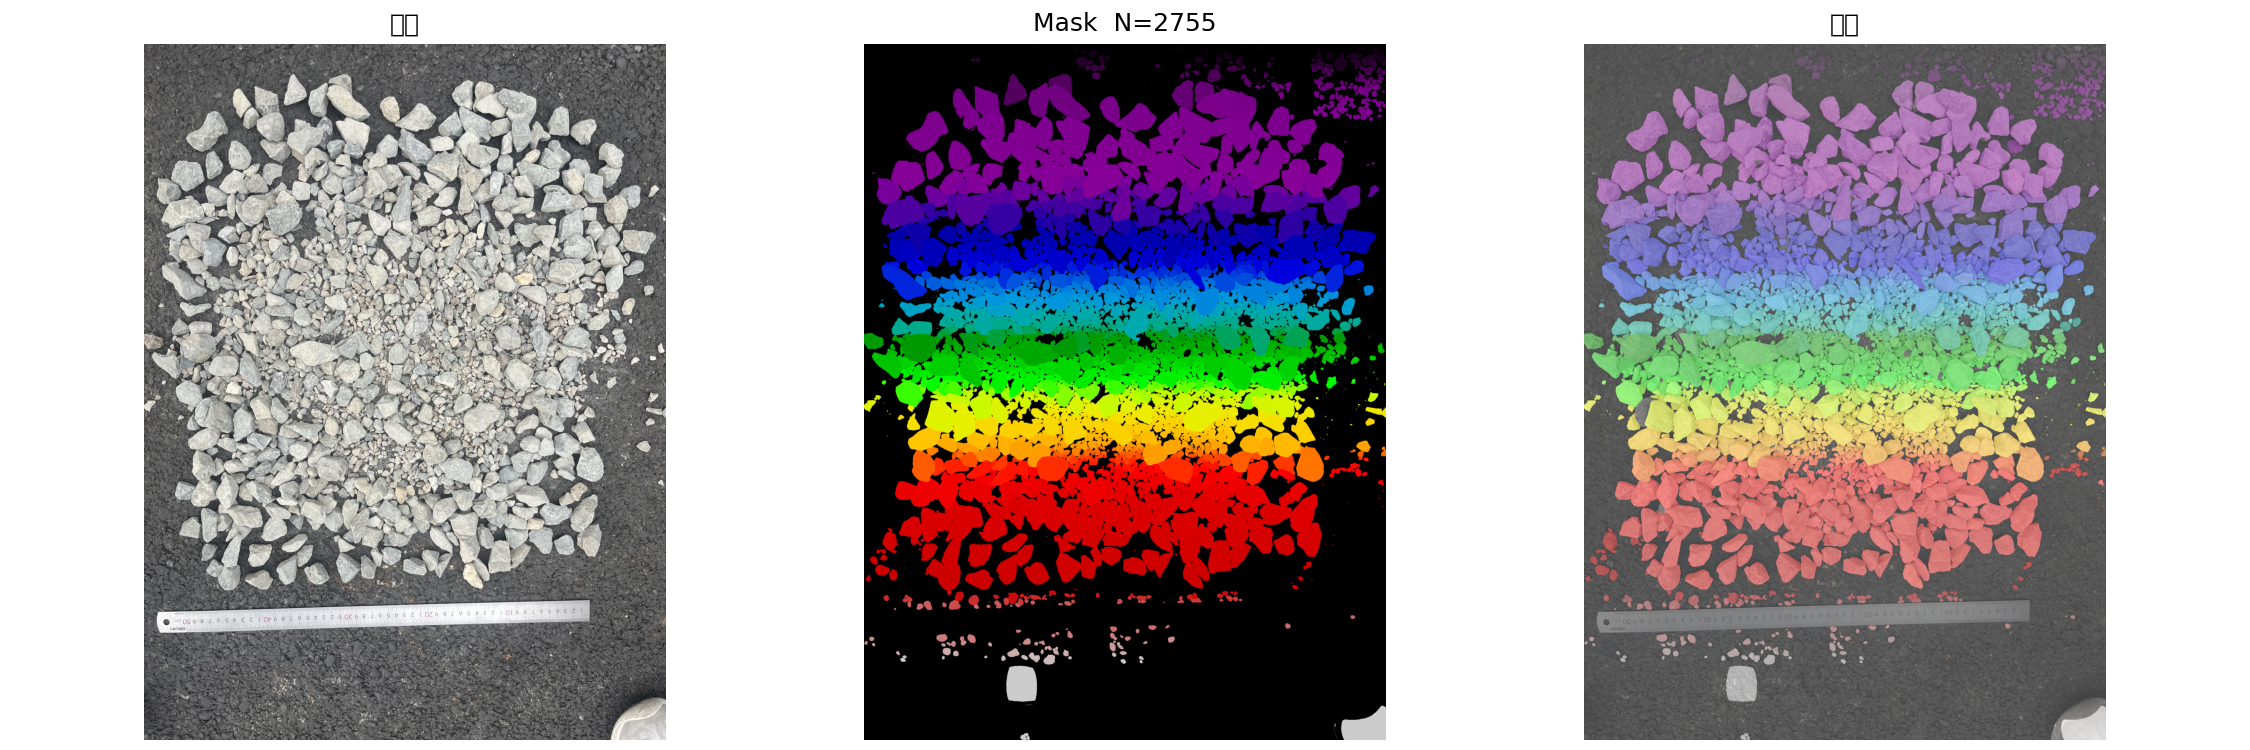
\includegraphics[width=0.86\linewidth]{agg_001_IG2_full_set_cp_SAM_pred_grains_re_scaled_detection_overview.png}
\caption{真实自然堆积样本的实例检测与粒径标注概览。可视化的主要作用是使最终级配能够回溯到具体实例，并快速发现 merge、split、漏检或明显尺度异常。}
\label{fig:r-demo-detection}
\end{figure}

\subsection{颗粒几何与任务特征}

对实例 mask $M_i$，系统提取面积 $A_i$、周长 $P_i$、凸包面积 $A_{\mathrm{conv},i}$、拟合椭圆长轴 $a_i$ 和短轴 $b_i$。长度经式\eqref{eq:r-scale}转换到毫米，面积按 $r^2$ 转换。面积等效直径定义为
\begin{equation}
 d_{\mathrm{eq},i}=2\sqrt{\frac{A_i}{\pi}},
\label{eq:r-deq}
\end{equation}
并计算三个无量纲形貌量
\begin{equation}
 \mathrm{AR}_i=\frac{b_i}{a_i},\qquad
 C_i=\frac{4\pi A_i}{P_i^2},\qquad
 S_i=\frac{A_i}{A_{\mathrm{conv},i}}.
\label{eq:r-shape}
\end{equation}
其中 AR 描述细长程度，$C$ 描述圆度，$S$ 描述相对于凸包的凹凸程度。这些量一方面参与后续筛分粒径映射，另一方面复用于形貌和异常分支，从而避免为每个任务建立彼此独立、难以解释的模型。

当前投影形貌规则以 AR、$C$ 和 $S$ 将颗粒划分为针片状候选、圆形、棱角状和普通四类；其中“针片状候选”只描述二维投影细长性，不能替代含厚度维度的规范针片状判定。异常分支以物理粒径和凸度做快速筛查：$d>50$~mm 标记为超限，$d<5$~mm 标记为过小候选，40--50~mm 且低凸度的目标仅标记为疑似泥团。前两类有明确几何定义，而泥团本质上是材质语义问题，因此当前几何规则只承担候选筛查，后续若需要可靠泥团识别，应加入颜色/纹理或小型裁剪分类器。

至此，图像已经被压缩为一组可追溯的毫米级颗粒描述 $\{\mathbf{x}_i\}$。但这些几何量仍然不是标准筛分结果：短轴是二维投影量，机械筛孔对应三维动态通过行为；同时图像按实例计数，而机械筛分按质量称重。下一节处理全文最关键的“筛分语义鸿沟”。

% ===== 4 筛分语义映射 =====
\section{从二维视觉到标准筛分级配}
\label{sec:r-sieve}

\subsection{二维视觉粒径不等于筛孔粒径}

机械筛分判断的是三维颗粒在振动和姿态变化过程中能否通过给定筛孔，而单目相机只能观测当前姿态下的二维投影。因此，某个二维长度可以作为筛分行为的代理，但不能未经验证地与筛孔尺寸画等号。图\ref{fig:r-sieve-semantics}示意了两者的物理差异：相机得到的是当前视角的投影椭圆和可见轮廓；机械筛分则允许颗粒在三维中旋转并寻找可通过筛孔的姿态，决定通过行为的尺度可能同时受短轴、厚度、形状和姿态影响。

\begin{figure}[t]
\centering
\begin{tikzpicture}[
  box/.style={rectangle,draw,rounded corners,minimum width=4.0cm,minimum height=2.1cm,align=center,font=\footnotesize},
  arr/.style={->,thick}
]
\node[box,fill=gray!7] (grain) {\begin{tikzpicture}[scale=0.7]
\draw[thick,rotate=15] (0,0) ellipse (1.25 and 0.72);
\draw[dashed,rotate=15] (0,0) ellipse (1.25 and 0.32);
\draw[<->] (-1.15,-0.95)--(1.15,-0.95) node[midway,below,font=\scriptsize] {三维尺寸与姿态};
\end{tikzpicture}\\真实颗粒};
\node[box,fill=blue!7,right=0.8cm of grain] (proj) {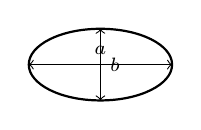
\begin{tikzpicture}[scale=0.7]
\draw[thick] (0,0) ellipse (1.3 and 0.65);
\draw[<->] (-1.3,0)--(1.3,0) node[midway,above,font=\scriptsize] {$a$};
\draw[<->] (0,-0.65)--(0,0.65) node[midway,right,font=\scriptsize] {$b$};
\end{tikzpicture}\\单目二维投影};
\node[box,fill=orange!8,right=0.8cm of proj] (sieve) {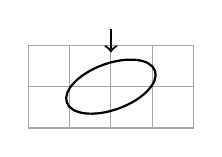
\begin{tikzpicture}[scale=0.7]
\draw[step=0.75cm,gray!70] (-1.5,-0.75) grid (1.5,0.75);
\draw[thick,rotate=20] (0,0) ellipse (0.85 and 0.42);
\draw[->,thick] (0,1.05)--(0,0.62);
\end{tikzpicture}\\动态筛孔通过行为};
\draw[arr] (grain)--node[above,font=\scriptsize]{成像}(proj);
\draw[arr] (proj)--node[above,font=\scriptsize]{需要校准映射}(sieve);
\end{tikzpicture}
\caption{二维视觉几何与机械筛分语义的差异。短轴 $b$ 是合理的低维代理，但投影中缺失的厚度和动态姿态决定其不能被先验地视为真实筛孔粒径。}
\label{fig:r-sieve-semantics}
\end{figure}

对于多数颗粒，投影短轴 $b_i$ 比长轴更接近潜在通过方向，因此本文把 $d=b$ 作为\textbf{无机械筛分真值时的可解释基线}；但扁平、细长和不规则颗粒仍会受到第三维厚度、姿态和轮廓形状影响。已有图像粒度研究同样表明，视觉尺寸与筛分/质量粒度之间需要额外映射，而不能只比较颗粒个数\cite{maiti2017massModel,mair2023automated}。

为在保持低数据需求的同时吸收平均系统偏差，本文构造筛分等效粒径
\begin{equation}
 d_i=\theta_1 b_i+\theta_2 d_{\mathrm{eq},i}+\theta_3,
\label{eq:r-sieve-d}
\end{equation}
其中 $b_i$ 描述较接近筛孔通过方向的线性尺度，$d_{\mathrm{eq},i}$ 引入投影面积信息，$\theta_3$ 用于吸收稳定的尺度偏移。当前演示采用 $\boldsymbol{\theta}=(1,0,0)$，即 $d=b$；这一设置是未校准基线，不是声称短轴已经等价于机械筛分粒径。

表\ref{tab:r-diameter-candidates}说明为什么把短轴、等效直径和低维组合都保留在实验设计中。若只比较最终组合模型，无法判断精度改善究竟来自面积信息还是参数自由度；因此正式消融应使用同一独立机械筛分测试集比较这些候选。选择低维显式模型而非直接训练高容量回归器，是因为配对机械筛分批次预计远少于普通视觉数据，且比赛答辩需要能够解释参数改变为何会使级配变粗或变细。

\begin{table}[t]
\centering
\caption{筛分粒径候选及其物理含义。真正优劣必须由独立机械筛分误差决定。}
\label{tab:r-diameter-candidates}
\footnotesize
\renewcommand{\arraystretch}{1.12}
\begin{tabular}{>{\raggedright\arraybackslash}p{2.8cm}>{\raggedright\arraybackslash}p{4.6cm}>{\raggedright\arraybackslash}p{5.5cm}}
\toprule
候选 & 优点 & 主要局限/验证目的 \\
\midrule
$d=b$ & 参数最少；接近潜在通过方向；可解释性最高 & 忽略投影面积与形状差异；作为物理基线 \\
$d=d_{\mathrm{eq}}$ & 同时利用两个方向的面积信息；对轮廓整体稳定 & 对细长/扁平颗粒可能高估可通过尺度；作为面积基线 \\
式\eqref{eq:r-sieve-d} & 线性融合短轴与面积，并允许统一偏移 & 需要配对筛分批次校准；验证低维组合是否降低测试误差 \\
端到端回归 & 理论容量高，可学习复杂非线性 & 配对数据需求高、可解释性弱；仅在低维模型残差明确后考虑 \\
\bottomrule
\end{tabular}
\end{table}

\subsection{从颗粒数量到质量相关统计}

即使 $d_i$ 能够很好地代表筛孔粒径，图像统计与机械筛分仍有第二个根本差异：前者天然给每个实例相同权重，后者通过称重得到质量比例。设颗粒尺度为 $d_i$，在密度近似一致、形状随尺寸统计上相似的假设下，颗粒质量随特征尺度近似按幂律增长，因此定义
\begin{equation}
 w_i=d_i^{\gamma}.
\label{eq:r-mass}
\end{equation}
默认 $\gamma=3$ 对应体积随线性尺度立方增长的基线直觉，但真实骨料的厚度比例和形貌可能随尺寸变化，故 $\gamma$ 与 $\boldsymbol{\theta}$ 一样需要由配对机械筛分数据校准，而不能作为普适常数。

在权重 $w_i$ 下，质量相关累计分布定义为
\begin{equation}
 F(d)=\frac{\sum_i w_i\,\mathbf{1}(d_i\le d)}{\sum_i w_i}.
\label{eq:r-cdf}
\end{equation}
特征粒径 $D_p$ 为使 $F(D_p)\ge p/100$ 的最小粒径；标准筛级质量占比则由相邻筛孔边界内的权重和归一化得到。本文使用 5、10、16、20、25、31.5 和 40~mm 作为主要粒级边界，使场景输出能够直接组织为与工程筛分相近的累计曲线和区间质量比例。

式\eqref{eq:r-mass}是全文最重要的统计转换之一。若所有实例等权，一个 4~mm 与一个 30~mm 颗粒各计作“1”；当 $\gamma=3$ 时，两者质量代理权重比约为 $(30/4)^3\approx422$，因此少量粗颗粒能够显著改变累计质量分布。这也是为什么数量型中位粒径通常远小于质量相关中位粒径。该现象本身能够验证“统计口径不可忽略”，但只有与机械筛分真值比较后，才能判断具体 $\gamma$ 是否正确。

参数的作用方向也是可解释的。增大 $\theta_1$ 会整体强化短轴贡献；增大 $\theta_2$ 会使投影面积较大的颗粒相对变粗；正的 $\theta_3$ 近似平移全部粒径；增大 $\gamma$ 则不改变单颗粒 $d_i$，而是提高粗颗粒在场景统计中的质量份额。正因为这些参数作用于不同层次，校准后仍应检查是否出现不合理的参数补偿，例如用过大的 $\gamma$ 去掩盖系统性偏小的 $d_i$。表\ref{tab:r-parameter-effects}给出参数变化时应观察的主要现象。

\begin{table}[t]
\centering
\caption{核心参数的作用层次、预期方向与诊断意义。}
\label{tab:r-parameter-effects}
\footnotesize
\renewcommand{\arraystretch}{1.12}
\begin{tabular}{>{\centering\arraybackslash}p{1.6cm}>{\raggedright\arraybackslash}p{3.5cm}>{\raggedright\arraybackslash}p{4.2cm}>{\raggedright\arraybackslash}p{3.9cm}}
\toprule
参数 & 作用对象 & 参数增大时的主要效应 & 需警惕的问题 \\
\midrule
$\theta_1$ & 个体粒径 & 强化短轴对 $d_i$ 的贡献 & 与尺度 $r$ 同方向补偿 \\
$\theta_2$ & 个体粒径 & 面积较大的颗粒相对增粗 & 对不规则/遮挡轮廓敏感 \\
$\theta_3$ & 个体粒径 & 近似统一平移粒径 & 对小颗粒相对影响更大 \\
$\gamma$ & 场景质量权重 & 粗颗粒质量份额增大，$D_p$ 常向粗端移动 & 可能放大 merge 和极端大实例 \\
\bottomrule
\end{tabular}
\end{table}

\subsection{机械筛分真值驱动的参数校准}

机械筛分在本文中不是被视觉方法“替代掉的对手”，而是定义下游筛分语义的物理锚点。对同一物理批次，先在规定成像条件下获取图像并保存预测粒级，再对该批材料执行标准机械筛分和逐筛称量，得到真实 $D_{10}^{\mathrm{GT}},D_{50}^{\mathrm{GT}},D_{90}^{\mathrm{GT}}$ 及完整筛孔质量分布。校准阶段只使用若干训练批次拟合 $\boldsymbol{\theta},\gamma$，独立测试批次在参数冻结后仅用于最终评价。

图\ref{fig:r-calibration-loop}强调“同批次配对”和“参数冻结”两个条件。前者保证视觉预测与机械真值描述的是同一批物料，而不是拿不同取样结果强行比较；后者保证测试批次只用于评价，避免根据最终答案重新选择参数。若一个物理批次拍摄多张图像，这些图像也必须整体属于校准或测试一侧，不能按图片随机拆分，否则会产生物理批次泄漏。

\begin{figure}[t]
\centering
\begin{tikzpicture}[
  node distance=0.6cm and 0.65cm,
  b/.style={rectangle,draw,rounded corners,minimum width=3.1cm,minimum height=0.85cm,align=center,font=\footnotesize},
  arr/.style={->,thick}, dash/.style={->,thick,dashed}
]
\node[b,fill=gray!8] (batch) {同一物理骨料批次};
\node[b,fill=blue!7,below left=0.65cm and 1.0cm of batch] (camera) {相机采集\\视觉逐颗粒预测};
\node[b,fill=yellow!12,below right=0.65cm and 1.0cm of batch] (sieve) {机械筛分\\逐筛称量真值};
\node[b,fill=orange!8,below=0.85cm of camera] (fit) {校准批次\\拟合 $\boldsymbol{\theta},\gamma$};
\node[b,fill=green!8,below=0.85cm of sieve] (test) {独立测试批次\\仅计算最终误差};
\node[b,fill=purple!7,below=0.8cm of fit,xshift=2.05cm] (freeze) {冻结参数\\正式测试/现场推理};
\draw[arr] (batch)--(camera); \draw[arr] (batch)--(sieve);
\draw[arr] (camera)--(fit); \draw[arr] (sieve)--(test);
\draw[dash] (sieve.west) -| (fit.east);
\draw[arr] (fit)--(freeze); \draw[arr] (freeze)--(test);
\end{tikzpicture}
\caption{机械筛分校准与独立测试协议。虚线表示校准批次的机械筛分真值参与参数拟合；独立测试批次不得反向参与参数选择。}
\label{fig:r-calibration-loop}
\end{figure}

当前代码对 $\theta_1,\theta_2\in[0,3]$、$\theta_3\in[-20,20]$~mm、$\gamma\in[1,5]$ 进行差分进化搜索。现有损失函数以三个特征粒径的相对误差为主：
\begin{equation}
\mathcal{L}=\frac{1}{B}\sum_{j=1}^{B}
\left(0.25r_{10,j}^2+0.50r_{50,j}^2+0.25r_{90,j}^2\right),\qquad
r_{p,j}=\frac{\widehat D_{p,j}-D_{p,j}^{\mathrm{GT}}}{\max(D_{p,j}^{\mathrm{GT}},10^{-6})}.
\label{eq:r-cal-loss}
\end{equation}
选择差分进化而非梯度法，是因为加权分位数和筛级归属对参数呈分段、非光滑变化。正式竞赛版本还应在独立测试中报告逐筛级质量占比误差，因为仅约束三个 $D_p$ 不能保证整条级配曲线一致。若数据量允许，可在校准损失中进一步加入筛级质量项；但无论损失如何变化，最终报告都应在未参与拟合的批次上统一评价。

\begin{table}[t]
\centering
\caption{筛分语义参数及其物理角色。}
\label{tab:r-sieve-params}
\footnotesize
\renewcommand{\arraystretch}{1.12}
\begin{tabular}{>{\raggedright\arraybackslash}p{2.2cm}>{\raggedright\arraybackslash}p{5.1cm}>{\raggedright\arraybackslash}p{5.7cm}}
\toprule
参数 & 作用 & 证据与冻结原则 \\
\midrule
$r$ & pixel $\rightarrow$ mm 的成像尺度 & 每次成像几何改变后由现场参考物重新测量 \\
$\theta_1,\theta_2,\theta_3$ & 二维几何 $\rightarrow$ 筛分等效粒径 & 用配对机械筛分校准；正式测试前冻结 \\
$\gamma$ & 粒径 $\rightarrow$ 质量代理权重 & 用配对机械筛分校准；正式测试前冻结 \\
筛孔边界 & 将连续 $d_i$ 聚合为工程粒级 & 由赛题/标准口径固定，不随测试样本调节 \\
\bottomrule
\end{tabular}
\end{table}

这一设计把两类容易混淆的“标定”彻底分开：$r$ 是本次相机几何的物理尺度标定，需要随设备位置变化重新测量；$\boldsymbol{\theta},\gamma$ 是视觉几何到筛分语义的统计校准，应在赛前利用机械筛分数据拟合后冻结。这样既允许现场恢复真实毫米尺度，又防止根据测试样本结果反向调参造成数据泄漏。

最终，本文的核心方法不是“Cellpose-SAM 识别石子”这一单点能力，而是式\eqref{eq:r-sieve-d}--\eqref{eq:r-cdf}组成的显式桥梁：预训练模型负责获得可用实例，尺度标定负责建立物理单位，筛分等效粒径负责处理二维投影与筛孔语义差异，质量权重负责处理数量统计与称重统计差异。下一节通过现有真实图像结果和拟定的机械筛分验证协议，分别检验这些环节当前能够支持哪些结论。

% ===== 5 实验与结果 =====
\section{实验设计与阶段性结果}
\label{sec:r-results}

\subsection{数据角色、证据协议与评价指标}

本文将实验分为三类证据。\textbf{功能演示}回答处理链能否从真实自然堆积图像稳定地产生实例、毫米几何、级配、形貌和异常输出；\textbf{软件一致性}通过合成单元测试检查数学定义和代码实现是否一致；\textbf{物理精度验证}则必须使用独立 ground truth，才能声明实例精度、筛分精度或形貌/异常准确率。三者不能互相替代，特别是没有机械筛分称量真值时，视觉级配曲线只能视为模型输出而非“准确率”。

表\ref{tab:r-evidence-roles}把当前已有数据与正式比赛仍需补充的数据分开。三张演示图用于确认完整数据链和展示场景差异；人工实例掩膜应覆盖普通区域与粘连/遮挡困难区域；机械筛分数据必须与成像使用同一物理批次；形貌与异常标签则用于附加任务。这样的拆分防止最常见的验证错误：用模型自己的另一个输出作为“真值”，或把同一物理批次的多张照片随机拆到训练和测试两侧。

\begin{table}[t]
\centering
\caption{评委版实验中不同数据的角色与当前状态。}
\label{tab:r-evidence-roles}
\footnotesize
\renewcommand{\arraystretch}{1.12}
\begin{tabular}{>{\raggedright\arraybackslash}p{3.0cm}>{\raggedright\arraybackslash}p{4.3cm}>{\raggedright\arraybackslash}p{4.2cm}>{\raggedright\arraybackslash}p{2.0cm}}
\toprule
数据 & 用途 & 关键输出/指标 & 状态 \\
\midrule
3 张自然堆积 demo & 端到端功能、行为性分析、可视化 & 实例数、$D_p$、粒级、形貌/异常 & 已有 \\
合成单元测试 & 数学定义与代码一致性 & 27 项测试是否通过 & 已有 \\
人工实例 mask & 上游实例精度与 merge/split & P/R/F1、IoU、merge/split & 待补 \\
配对机械筛分批次 & $\boldsymbol{\theta},\gamma$ 校准与独立筛分评价 & $D_p$ 误差、逐筛级误差、曲线误差 & 关键缺口 \\
人工形貌/异常标签 & 附加能力外部有效性 & Macro-F1、P/R/F1 & 待补 \\
完整现场演练 & 30~min 工程约束 & 端到端 wall-clock time、失败恢复 & 待实测 \\
\bottomrule
\end{tabular}
\end{table}

最终正式实验应围绕同一物理批次建立配对证据：相机分支产生视觉预测，机械筛分分支产生逐筛质量真值。校准批次用于拟合 $\boldsymbol{\theta},\gamma$；独立测试批次在参数冻结后计算
\begin{equation}
 E_{D_p}=\left|\widehat D_p-D_p^{\mathrm{GT}}\right|,
 \qquad
 \mathrm{MAE}_{\mathrm{sieve}}=\frac{1}{K}\sum_{k=1}^{K}\left|\widehat P_k-P_k^{\mathrm{GT}}\right|.
\label{eq:r-metrics}
\end{equation}
还应同时报告相对 $D_p$ 误差和累计通过率曲线，以避免单一指标掩盖局部筛级偏差。实例识别使用人工实例 mask 报告 Precision/Recall/F1、IoU 及 merge/split；二维形貌和异常分别使用人工标签报告 Macro-F1 或 Precision/Recall。工程性能按完整 SOP 的 wall-clock time 评价，而不是只统计神经网络前向时间。

实验采样还需要覆盖真正可能改变误差结构的场景变量，而不是只增加相似照片数量。至少应包含偏细、连续和偏粗级配；低/中/高接触程度；不同位置与轻度光照变化；以及人为加入的超限块和泥团候选。若最终机械筛分批次数量有限，宁可保证物理批次之间的级配差异和严格独立测试，也不应通过同一批材料拍很多相似图片制造虚假的大样本量。

\subsection{真实图像功能演示与场景差异}

当前仓库包含 \texttt{agg\_001}、\texttt{agg\_005} 和 \texttt{agg\_029} 三张自然堆积演示图像，分辨率均为 3024$\times$4032，使用已写入产物的尺度 0.208~mm/px。三张图在当前基线 $\boldsymbol{\theta}=(1,0,0)$、$\gamma=3$ 下共检测 3858 个实例，并生成逐颗粒几何表、筛分等效粒径、质量代理级配、形貌/异常标签及可视化。表\ref{tab:r-demo-main}汇总正常实例口径下的当前输出。由于参数尚未用本赛题配对机械筛分批次校准，这些 $D_p$ 只能解释为\textbf{当前视觉质量代理预测}。

\begin{table}[t]
\centering
\caption{三张自然堆积演示样本的当前视觉质量代理输出。}
\label{tab:r-demo-main}
\footnotesize
\renewcommand{\arraystretch}{1.12}
\begin{tabular}{lrrrrll}
\toprule
样本 & 实例数 & 正常实例 & $D_{10}$ & $D_{50}$ & $D_{90}$ & 主粒级 \\
 & & & \multicolumn{3}{c}{/ mm} & \\
\midrule
\texttt{agg\_001} & 1924 & 1193 & 11.1 & 23.6 & 30.6 & 25--31.5~mm（34.2\%） \\
\texttt{agg\_005} & 968 & 703 & 15.6 & 27.5 & 38.0 & 25--31.5~mm（29.7\%） \\
\texttt{agg\_029} & 966 & 520 & 6.7 & 14.6 & 30.6 & 5--10~mm（32.7\%） \\
\bottomrule
\end{tabular}
\end{table}

三张场景得到明显不同的预测结构：\texttt{agg\_005} 粗粒尾部更强，\texttt{agg\_029} 则明显偏细，$D_{50}$ 排序为 \texttt{agg\_029}<\texttt{agg\_001}<\texttt{agg\_005}。这支持“同一处理链能将不同真实场景转换为非退化的场景级级配描述”，但不能说明哪条曲线最接近机械筛分。图\ref{fig:r-three-gsd}进一步把三个场景的数量/质量代理输出并列展示，可以看到差异不是由一个汇总数字产生，而是在完整分布形状上存在。

\begin{figure}[t]
\centering
\begin{subfigure}{0.32\linewidth}
\centering
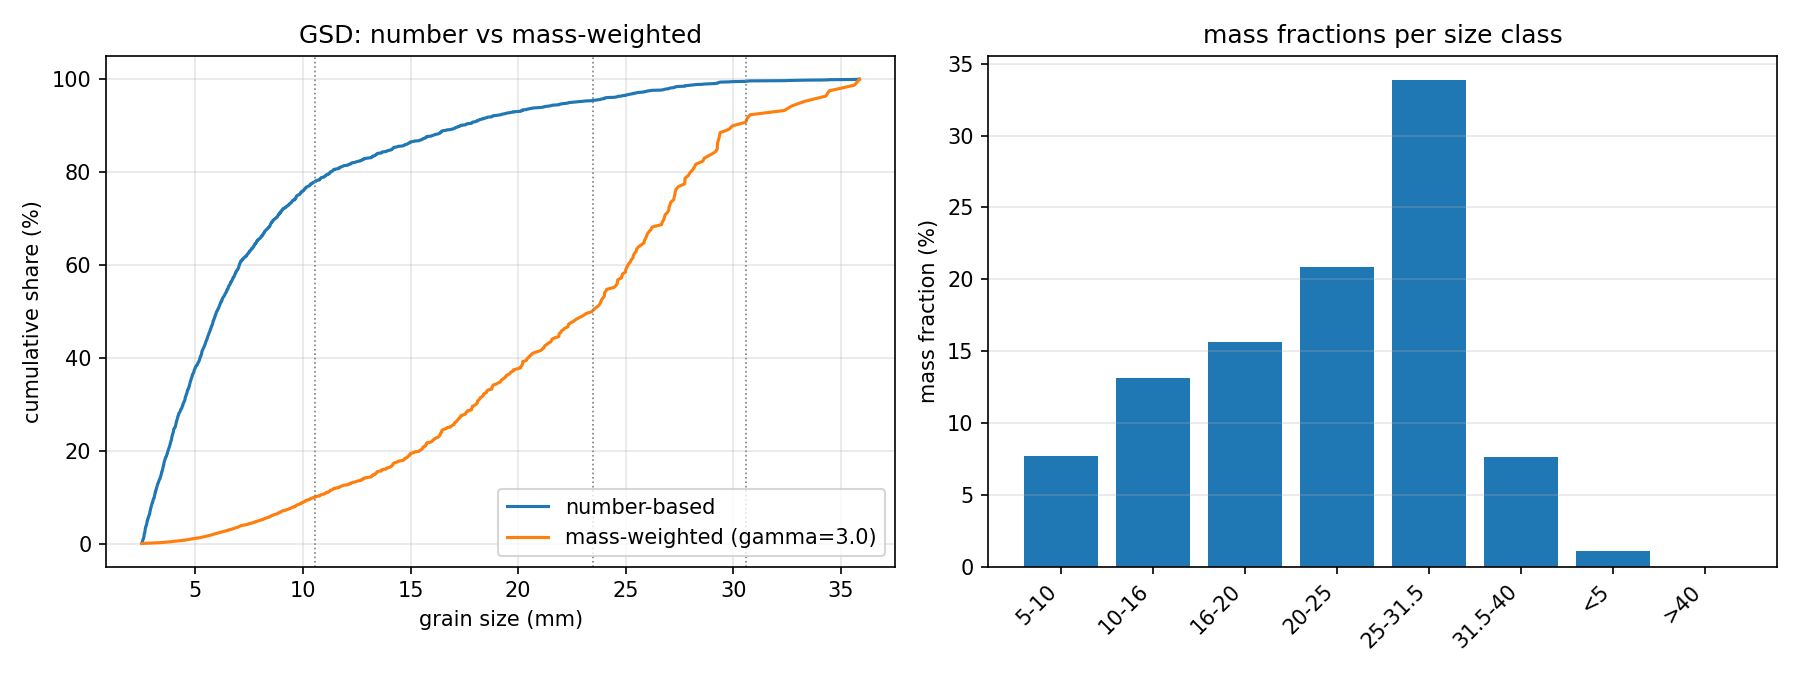
\includegraphics[width=\linewidth]{agg_001_IG2_full_set_cp_SAM_pred_grains_re_scaled_gsd_comparison.png}
\caption{\texttt{agg\_001}}
\end{subfigure}\hfill
\begin{subfigure}{0.32\linewidth}
\centering
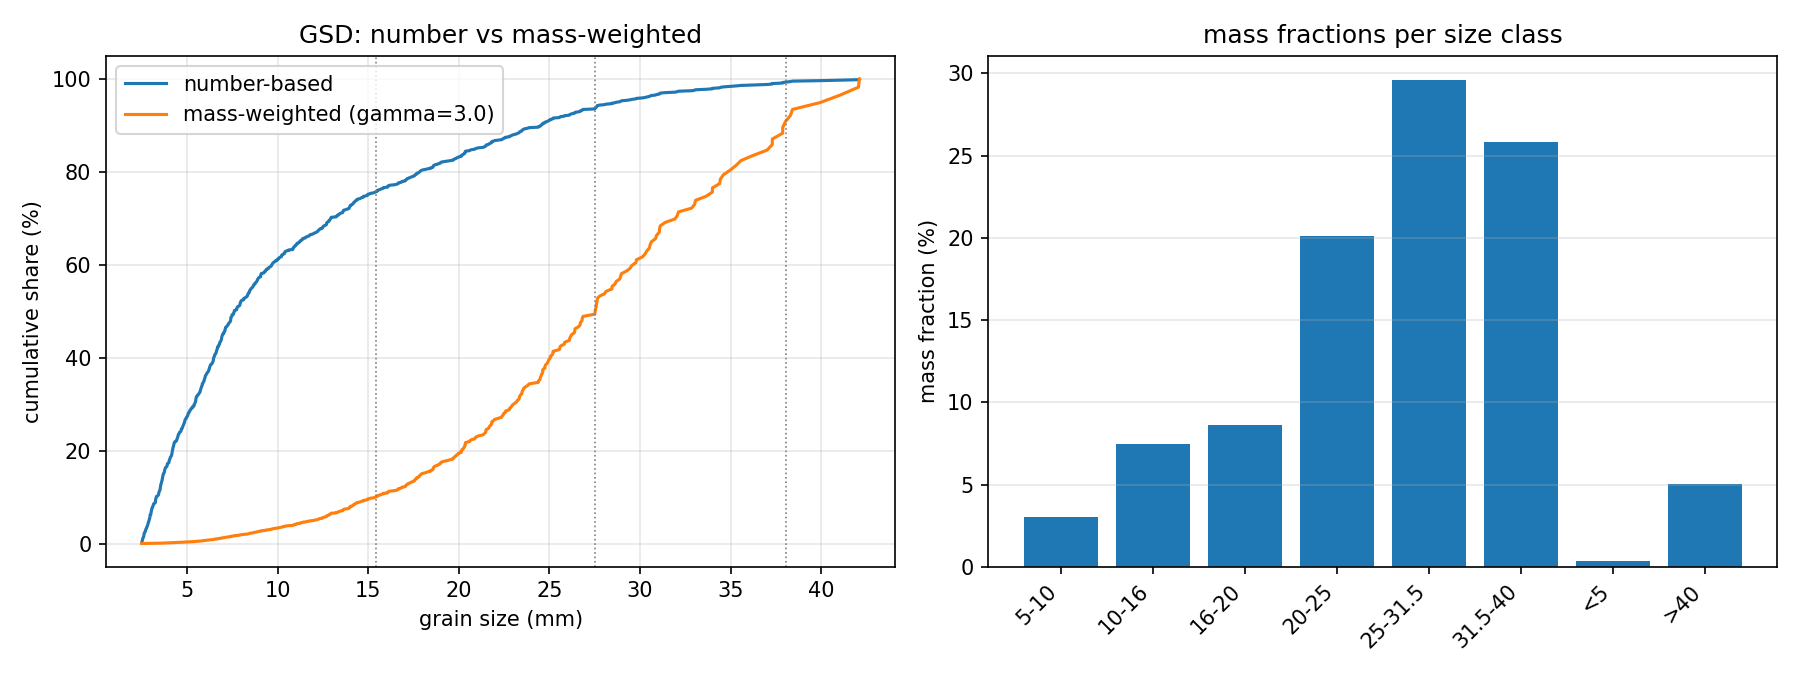
\includegraphics[width=\linewidth]{agg_005_IG2_full_set_cp_SAM_pred_grains_re_scaled_gsd_comparison.png}
\caption{\texttt{agg\_005}}
\end{subfigure}\hfill
\begin{subfigure}{0.32\linewidth}
\centering
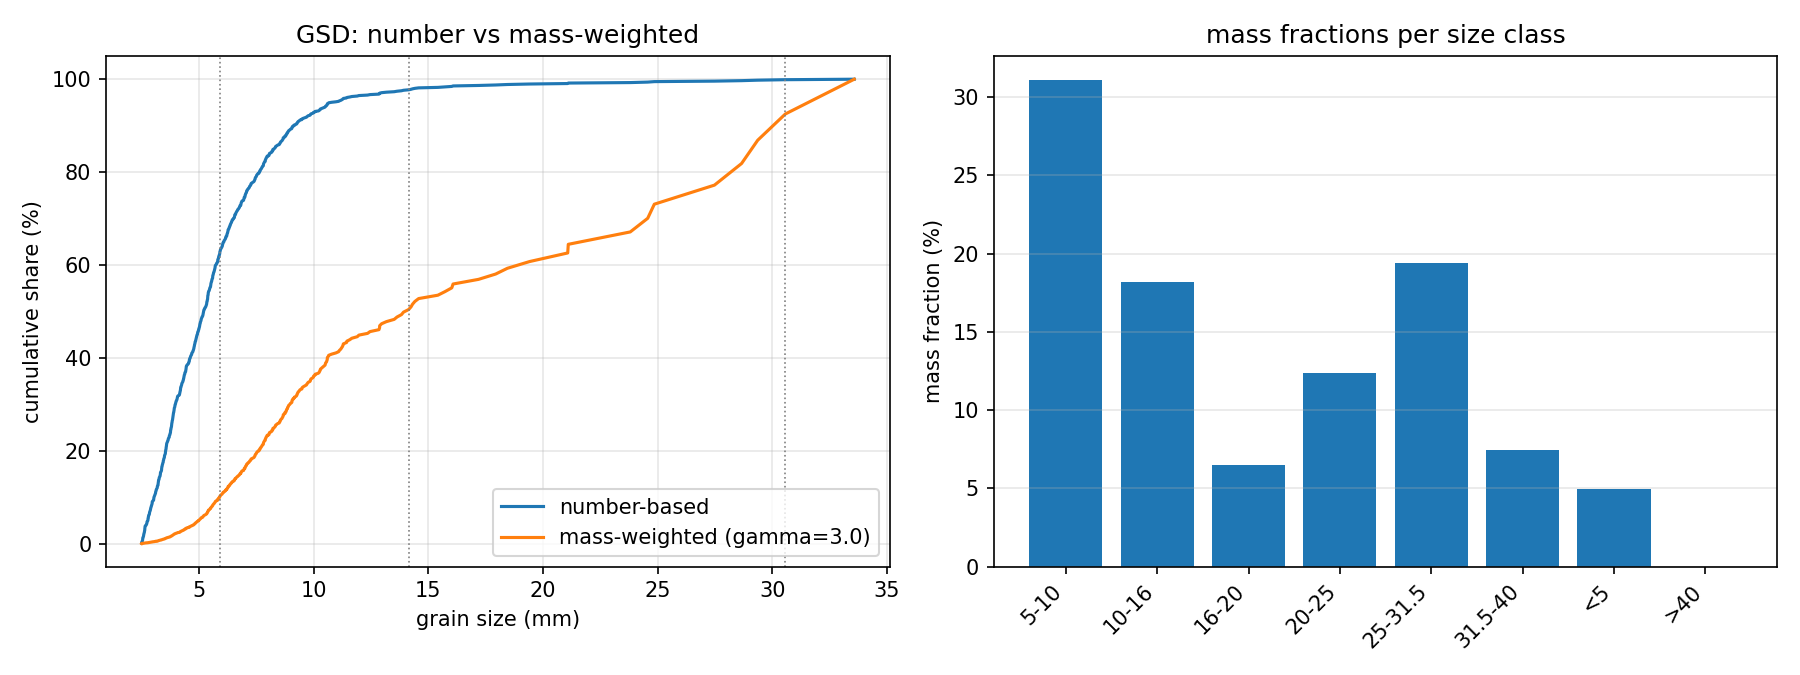
\includegraphics[width=\linewidth]{agg_029_IG2_full_set_cp_SAM_pred_grains_re_scaled_gsd_comparison.png}
\caption{\texttt{agg\_029}}
\end{subfigure}
\caption{三张演示样本的数量型与质量代理型粒径分布。图中没有机械筛分真值，因此用于比较场景行为和统计口径，不作为物理准确率曲线。}
\label{fig:r-three-gsd}
\end{figure}

从逐筛质量代理比例也能看出场景结构差异。\texttt{agg\_001} 的 20--31.5~mm 合计约 55.3\%，\texttt{agg\_005} 的 25--40~mm 约 55.6\%，而 \texttt{agg\_029} 的 5--16~mm 约 51.9\%。这些比例来自同一计算规则，因此能够用于检查实现是否对不同输入给出一致口径；但它们只有在机械筛分配对后才可转化为“预测误差”。

\subsection{数量统计与质量代理：核心行为性证据}

当前最稳定且最重要的观察是：\textbf{数量型粒径分布与质量代理型粒径分布存在显著差异}。表\ref{tab:r-number-mass}给出异常处理前、基于全部检测实例的分位数。三张图的数量型 $D_{50}$ 仅为 5.2--7.6~mm，而采用 $w=d^3$ 后移动到 14.1--27.5~mm；方向在三个场景中一致。

\begin{table}[t]
\centering
\caption{数量型与质量代理型分位数比较。该结果证明统计口径影响显著，不证明 $\gamma=3$ 已获得物理校准。}
\label{tab:r-number-mass}
\footnotesize
\renewcommand{\arraystretch}{1.12}
\begin{tabular}{lrrrrrr}
\toprule
& \multicolumn{3}{c}{数量型 / mm} & \multicolumn{3}{c}{质量代理 / mm} \\
\cmidrule(lr){2-4}\cmidrule(lr){5-7}
样本 & $D_{10}$ & $D_{50}$ & $D_{90}$ & $D_{10}$ & $D_{50}$ & $D_{90}$ \\
\midrule
\texttt{agg\_001} & 3.1 & 6.0 & 17.3 & 10.6 & 23.5 & 30.6 \\
\texttt{agg\_005} & 3.3 & 7.6 & 24.5 & 15.4 & 27.5 & 38.0 \\
\texttt{agg\_029} & 3.0 & 5.2 & 9.2 & 5.9 & 14.1 & 30.6 \\
\bottomrule
\end{tabular}
\end{table}

该变化可由式\eqref{eq:r-mass}直接解释：自然堆积图中小实例数量很多，但其单颗粒质量贡献较低；少量粗颗粒虽然在个数中占比小，却在幂次权重下显著影响累计质量。以 \texttt{agg\_001} 为例，当前 $<5$~mm 实例占检测数量的 38.0\%，剔除这些实例后质量代理 $D_{50}$ 仅由 23.50~mm 变为 23.56~mm，说明“大量小实例”不必然意味着“大量质量”。相反，错误 merge 产生的少量粗目标会被 $d^{\gamma}$ 放大，因此独立实例边界对高分位质量级配尤为关键。

\texttt{agg\_029} 提供了另一个有用现象：其正常实例仅占检测数的 53.8\%，过小候选数量最多，但正常口径下质量代理 $D_{90}$ 仍达到 30.6~mm。换言之，数量端“看起来很细”和质量端仍存在粗颗粒贡献可以同时成立。这正是机械筛分按质量计量与机器视觉按目标计数之间的统计差异，也是本文必须显式建立质量映射而非直接报告实例直方图的原因。

需要区分两个结论：现有结果足以支持“不能忽略质量口径”；但 $\gamma$ 越大本来就会推动分布向粗粒移动，因此不能仅凭曲线看起来更合理就选定 $\gamma=3$。只有当某个 $\gamma$ 在独立机械筛分测试上降低式\eqref{eq:r-metrics}的误差时，才能把它称为更好的物理质量模型。

\subsection{投影形貌与异常候选}

当前几何规则在三张图上均产生了非退化的投影形貌分布，具体比例见表\ref{tab:r-shape-results}。普通类占 55.0\%--64.1\%，针片状候选约 14.0\%--20.9\%；\texttt{agg\_005} 的针片状候选比例最高，而 \texttt{agg\_029} 的圆形比例相对较高。这些差异说明 AR、圆度和凸度能够把场景中的二维轮廓组织成可检查统计，但没有人工/量规 ground truth 时不能进一步解释为材料真实针片状率。

\begin{table}[t]
\centering
\caption{三张演示样本的投影形貌规则输出（占全部检测实例比例，\%）。}
\label{tab:r-shape-results}
\footnotesize
\begin{tabular}{lrrrr}
\toprule
样本 & 针片状候选 & 圆形 & 棱角状 & 普通 \\
\midrule
\texttt{agg\_001} & 16.3 & 8.0 & 16.4 & 59.3 \\
\texttt{agg\_005} & 20.9 & 6.6 & 17.6 & 55.0 \\
\texttt{agg\_029} & 14.0 & 11.0 & 11.0 & 64.1 \\
\bottomrule
\end{tabular}
\end{table}

图\ref{fig:r-shape-montage}以 \texttt{agg\_001} 为例展示四类高亮结果。图的价值在于检查规则是否定位到了与定义一致的轮廓类型，而不是用视觉印象代替准确率。例如，针片状候选应主要集中于低 AR 的细长投影；圆形应同时具有较高圆度和凸度。若高亮区域明显不符合这些定义，优先应检查实例 mask 和阈值实现，而不是直接解读最终比例。

\begin{figure}[t]
\centering
\begin{subfigure}{0.24\linewidth}\centering

\includegraphics[width=\linewidth]{agg_001_IG2_full_set_cp_SAM_pred_grains_re_scaled_shape_needle_flaky.png}
\caption{针片状候选}
\end{subfigure}\hfill
\begin{subfigure}{0.24\linewidth}\centering

\includegraphics[width=\linewidth]{agg_001_IG2_full_set_cp_SAM_pred_grains_re_scaled_shape_round.png}
\caption{圆形}
\end{subfigure}\hfill
\begin{subfigure}{0.24\linewidth}\centering

\includegraphics[width=\linewidth]{agg_001_IG2_full_set_cp_SAM_pred_grains_re_scaled_shape_angular.png}
\caption{棱角状}
\end{subfigure}\hfill
\begin{subfigure}{0.24\linewidth}\centering

\includegraphics[width=\linewidth]{agg_001_IG2_full_set_cp_SAM_pred_grains_re_scaled_shape_regular.png}
\caption{普通}
\end{subfigure}
\caption{\texttt{agg\_001} 的二维投影形貌高亮。类别由几何阈值产生，图像用于规则可解释性检查，不替代专家形貌 ground truth。}
\label{fig:r-shape-montage}
\end{figure}

异常分支的当前输出见表\ref{tab:r-anomaly-results}。三张图均未触发 $>50$~mm oversized 或疑似泥团规则，主要触发的是 $<5$~mm 小目标。该结果不能说明系统对 oversized 或泥团“零误报且完全正确”，更准确的结论是：\textbf{当前三张演示数据不包含足以检验这两个分支的阳性证据。} 正式测试应主动构造正常骨料、已知 $>50$~mm 大块和泥团/非骨料异物混合样本，分别计算 Precision/Recall，而不是等待随机场景恰好出现异常。

\begin{table}[t]
\centering
\caption{演示样本的异常规则输出（实例数）。}
\label{tab:r-anomaly-results}
\footnotesize
\begin{tabular}{lrrrr}
\toprule
样本 & 正常 & $>50$~mm & $<5$~mm & 疑似泥团 \\
\midrule
\texttt{agg\_001} & 1193 & 0 & 731 & 0 \\
\texttt{agg\_005} & 703 & 0 & 265 & 0 \\
\texttt{agg\_029} & 520 & 0 & 446 & 0 \\
\bottomrule
\end{tabular}
\end{table}

\subsection{软件一致性与工程时序}

仓库为筛分等效粒径、质量权重、加权分位数、形貌规则、异常优先级和报告生成提供了 27 项合成单元测试，当前记录全部通过。表\ref{tab:r-software-tests}说明这些测试能够证明和不能证明什么。特别是，合成数据可以构造已知 $\boldsymbol{\theta},\gamma$ 并检查优化器是否恢复接近设定值，这证明参数拟合路径在数学上可运行；它并不证明真实骨料确实服从该模型。

\begin{table}[t]
\centering
\caption{竞赛层软件测试的证据范围。}
\label{tab:r-software-tests}
\footnotesize
\renewcommand{\arraystretch}{1.12}
\begin{tabular}{>{\raggedright\arraybackslash}p{3.2cm}>{\raggedright\arraybackslash}p{5.0cm}>{\raggedright\arraybackslash}p{5.2cm}}
\toprule
模块 & 测试关注点 & 不能替代的现实验证 \\
\midrule
筛分等效与校准 & 粒径公式、质量权重、分位数、合成参数恢复 & 真实二维粒径与机械筛孔的对应关系 \\
形貌 & AR/$C$/$S$ 阈值与优先级逻辑 & 专家/量规形貌准确率 \\
异常 & oversized/undersized/泥团候选规则边界 & 真实异常 Precision/Recall \\
报告 & JSON/表格字段、正常口径与异常剔除一致性 & 现场输入质量和外部物理准确率 \\
\bottomrule
\end{tabular}
\end{table}

历史运行记录约为实例分割 17~s、几何测量 9~s、筛分统计 $<1$~s，即算法阶段约 27~s/张。计算本身因此不是 30~min 约束下的主要瓶颈；更可能占用现场时间的是设备就位、尺度确认、采集质检、模型首次加载、结果目检和一次失败恢复。基于这一判断，第\ref{sec:r-deploy}节把 30~min 预算分配给完整操作链，而不是将“27 秒”直接写成系统总耗时。

\subsection{最终机械筛分验证与最小消融矩阵}

当前最关键的实验缺口是：三张演示样本没有配对提交逐筛机械称量数据。因此本版本不填写机械筛分准确率，也不把未校准 $D_p$ 作为竞赛精度结论。正式测试应至少建立若干配对批次，其中一部分用于拟合参数，另一部分完全隔离为测试集。独立测试中至少报告：三个 $D_p$ 的绝对/相对误差、逐筛级质量占比或累计通过率误差，以及各批次均值与离散程度。表\ref{tab:r-physical-template}给出最终报告应替换的结果位置；当前保持“待测”比填入视觉自比较数字更符合证据逻辑。

\begin{table}[t]
\centering
\caption{独立机械筛分测试的最终结果模板。获得同批逐筛称量后直接回填。}
\label{tab:r-physical-template}
\footnotesize
\renewcommand{\arraystretch}{1.12}
\begin{tabular}{lrrrrr}
\toprule
测试批次 & $|\Delta D_{10}|$ & $|\Delta D_{50}|$ & $|\Delta D_{90}|$ & 筛级 MAE & 曲线/累计误差 \\
 & \multicolumn{3}{c}{/ mm} & / percentage point & \\
\midrule
Test-1 & 待测 & 待测 & 待测 & 待测 & 待测 \\
Test-2 & 待测 & 待测 & 待测 & 待测 & 待测 \\
Test-3 & 待测 & 待测 & 待测 & 待测 & 待测 \\
\midrule
平均 & 待测 & 待测 & 待测 & 待测 & 待测 \\
\bottomrule
\end{tabular}
\end{table}

同时需要用同一独立测试集完成表\ref{tab:r-ablation-matrix}的最小消融。实验顺序应回答四个因果问题：短轴是否比面积等效直径更接近筛分；二者组合是否进一步降低误差；质量加权是否比数量等权更接近称重结果；机械筛分校准是否能在未见批次上继续降低误差。异常剔除则用于检查极端误检是否通过 $d^\gamma$ 放大并污染最终级配。

\begin{table}[t]
\centering
\caption{正式物理验证的最小消融矩阵。所有行必须在同一独立测试批次上比较。}
\label{tab:r-ablation-matrix}
\footnotesize
\renewcommand{\arraystretch}{1.1}
\begin{tabular}{>{\centering\arraybackslash}p{0.8cm}>{\raggedright\arraybackslash}p{4.0cm}>{\raggedright\arraybackslash}p{4.6cm}>{\raggedright\arraybackslash}p{4.0cm}}
\toprule
编号 & 设置 & 回答的问题 & 主要比较指标 \\
\midrule
A & $d=b$，数量等权 & 最简视觉粒径/计数基线有多大语义差距？ & $D_p$、筛级 MAE \\
B & $d=b$，固定 $\gamma=3$ & 仅引入质量口径是否改善？ & B vs. A \\
C & $d=d_{\mathrm{eq}}$，同一 $\gamma$ & 面积尺度还是短轴更接近筛孔？ & C vs. B \\
D & 式\eqref{eq:r-sieve-d}，固定 $\gamma$ & 低维几何融合是否有效？ & D vs. B/C \\
E & 式\eqref{eq:r-sieve-d}，校准 $\gamma$ & 质量指数校准是否具有独立收益？ & E vs. D \\
F & E + 异常/质量控制 & 极端实例过滤能否降低粗端误差？ & F vs. E；失败案例 \\
\bottomrule
\end{tabular}
\end{table}

真正有解释力的结论应表述为“某设计使机械筛分独立测试误差降低多少”，而不是“参数变化后曲线移动了多少”。若 E 相比 D 没有稳定收益，则应保留更简单的固定质量模型；若 D 相比 $b$ 基线没有改善，则不应为了方法复杂度保留额外参数。换言之，最终系统结构也应由物理验证裁剪，而不是默认所有提出的模块都必须保留。在获得这些 ground truth 之前，本文明确保留证据边界，比给出未经验证的高准确率更能反映系统当前真实成熟度。

% ===== 6 工程部署与边界 =====
\section{现场部署、误差边界与改进优先级}
\label{sec:r-deploy}

\subsection{现场系统与硬件条件}

现场部署的首要目标不是追求单模块极限速度，而是保证\textbf{几何可追溯、视觉可质检、参数可冻结、结果可复现}。因此，硬件选择不以某个品牌或型号为核心，而以是否能够稳定恢复算法所依赖的物理条件为核心。固定俯视相机需要为 5--40~mm 主粒级提供足够像素覆盖；低畸变镜头和刚性支架保证一次测试内成像几何不漂移；深色哑光承载面与漫射照明降低硬阴影、高光和背景纹理造成的实例边界错误；与骨料测量面尽量共面的标尺或平面标记提供本次尺度锚点；CUDA GPU 则主要用于压缩 Cellpose-SAM 推理时间，使现场时间余量集中在标定、质检与失败恢复上。

表\ref{tab:r-hardware}给出适合本方案的工程配置及其与最终误差的关系。约 12~MP、固定焦距镜头等数值是当前推荐条件，而不是方法成立的唯一型号要求。若现场更换相机或镜头，应重新验证最小颗粒像素覆盖、透视与畸变，而不能仅因为“像素总数更高”就默认测量更准确。对静态自然堆积场景，普通固定曝光相机即可；若扩展到输送带，则全局快门和更短曝光优先级显著提高，因为运动模糊会直接改变轮廓几何。

\begin{table}[t]
\centering
\caption{推荐硬件条件及其与算法误差的直接关系。}
\label{tab:r-hardware}
\footnotesize
\renewcommand{\arraystretch}{1.12}
\begin{tabular}{>{\raggedright\arraybackslash}p{2.0cm}>{\raggedright\arraybackslash}p{4.0cm}>{\raggedright\arraybackslash}p{6.6cm}}
\toprule
模块 & 推荐条件 & 影响与现场验收重点 \\
\midrule
相机 & 约 12~MP 或更高；固定曝光；动态场景优先全局快门 & 保证 5~mm 附近仍有足够像素覆盖；检查无明显运动模糊、过曝或欠曝 \\
镜头/支架 & 固定焦距、低畸变、刚性俯视安装 & 保持一次测试内 mm/px 稳定；焦距、高度改变后必须重新标定 \\
承载面 & 深色、哑光、尽量平整 & 降低背景纹理和高光对边界的干扰；减少参考面与骨料面高度差 \\
照明 & 大面积漫射、亮度稳定 & 减少接触颗粒之间的硬阴影连接，降低 merge 风险 \\
尺度参考 & 标尺或已知尺寸平面标记，与测量面尽量共面 & 建立 pixel$\rightarrow$mm 锚点；多位置读数应基本一致 \\
计算设备 & 支持 CUDA 的 NVIDIA GPU & 缩短预训练模型推理并为现场重拍/复跑留出时间余量 \\
\bottomrule
\end{tabular}
\end{table}

软件链分为两个阶段。第一阶段由 \texttt{imagegrains} 完成实例分割、几何测量和毫米尺度写入，输出 mask、实例可视化及逐颗粒 CSV；第二阶段由 \texttt{aggregate\_screening} 读取逐颗粒表，计算筛分等效粒径、质量级配、形貌、异常与场景级报告。两阶段解耦后，如果上游实例已经通过质检，修改报告或重算下游统计不需要再次执行神经网络推理。正式比赛使用的模型版本、$\boldsymbol{\theta}$、$\gamma$ 和规则阈值在赛前冻结，现场只允许根据本次相机几何重新测量尺度 $r$。

\subsection{30 min 操作闭环与分层质检}

表\ref{tab:r-sop}给出面向 30~min 约束的操作预算。该表是工程上限而不是把历史 27~s/张算法时间简单外推为最终结论；正式赛前应完整演练并记录真实 wall-clock time。流程中特意保留重拍/复跑余量，因为尺度标错或整片 merge 一旦进入下游，会同时污染多个输出，现场尽早失败并恢复比事后解释异常数字更可靠。

\begin{table}[t]
\centering
\caption{评委版保留的 30~min 现场 SOP。}
\label{tab:r-sop}
\footnotesize
\renewcommand{\arraystretch}{1.12}
\begin{tabular}{>{\centering\arraybackslash}p{1.0cm}>{\raggedright\arraybackslash}p{3.2cm}>{\centering\arraybackslash}p{1.6cm}>{\raggedright\arraybackslash}p{7.2cm}}
\toprule
步骤 & 操作 & 预算 & 完成判据 \\
\midrule
1 & 设备就位、视场与照明 & 4~min & 目标完整入镜、相机固定、无明显硬阴影/模糊 \\
2 & 尺度标定 & 3~min & 获得本场景 mm/px；多位置参考无明显冲突 \\
3 & 采集与快速质检 & 3~min & 图像清晰、参考物共面且可读取 \\
4 & 分割与几何测量 & 5~min & 生成实例 mask/CSV；无大面积 merge 或数量级异常 \\
5 & 筛分、形貌、异常分析 & 2~min & 生成场景 summary、级配曲线和可视化 \\
6 & 结果质检与必要复跑 & 5~min & 尺度、轴长、实例和级配量级一致；必要时重拍/复跑固定配置 \\
7 & 导出与核对 & 3~min & 参数、逐颗粒表、场景报告和图像同时留存 \\
-- & 故障余量 & 5~min & 应对设备连接、模型加载或一次重拍 \\
\bottomrule
\end{tabular}
\end{table}

现场质检被设计为三个逐层门槛。\textbf{采集门槛}在神经网络推理前检查视场、曝光、清晰度、参考物和严重遮挡；这一层失败时直接重拍，因为输入证据本身已经不足。\textbf{实例门槛}在推理后检查 composite/overlay，重点寻找大面积 merge、异常碎裂、边缘截断和明显漏检；这一层失败时首先判断原因是否来自图像质量，若是则回到采集，否则只能按预先冻结的备用分割配置复跑，不能根据最终 $D_{50}$ 是否“好看”来临时调模型。\textbf{物理/报告门槛}检查参考长度反算、轴长量级、异常比例、筛级总和和输出文件完整性；这一层失败时停止提交，先定位尺度或数据链错误。

表\ref{tab:r-recovery}把几类最可能发生的现场异常转换为明确恢复动作。这里的核心原则是\textbf{根据中间证据决定是否重拍/复跑，而不是根据期望答案反向调参}。如果只看到最终级配曲线而没有实例和尺度证据，就无法区分“样品本来偏粗”和“模型整片 merge”；因此中间可视化不是展示附件，而是现场质量控制的一部分。

\begin{table}[t]
\centering
\caption{现场失败信号、原因判别与恢复动作。}
\label{tab:r-recovery}
\footnotesize
\renewcommand{\arraystretch}{1.11}
\begin{tabular}{>{\raggedright\arraybackslash}p{3.0cm}>{\raggedright\arraybackslash}p{3.7cm}>{\raggedright\arraybackslash}p{4.1cm}>{\raggedright\arraybackslash}p{2.3cm}}
\toprule
失败信号 & 优先检查原因 & 恢复动作 & 是否允许改模型参数 \\
\midrule
参考物模糊/尺度读数冲突 & 焦点、共面性、相机倾斜、镜头畸变 & 重拍或调整姿态；重新计算 $r$ & 否 \\
大面积整片 merge & 硬阴影、曝光、严重接触或域失配 & 优先改善采集并重拍；仍失败再用赛前冻结备用配置 & 仅冻结方案 \\
大量细碎 split & 分辨率、纹理、高光、后处理下限 & 检查图像质量；按冻结最小实例规则复跑 & 不临场搜索 \\
轴长方向/量级明显异常 & 错 CSV、旧 resolution、截断实例 & 核对 batch id 与尺度；必要时重跑测量 & 否 \\
$D_p$ 与场景观感突变 & merge、极端异常、质量权重输入错误 & 向上检查实例和逐颗粒表，不因结果预期改 $\gamma$ & 否 \\
输出文件缺失/不一致 & 路径、上一批文件混用、流程中断 & 从最近通过质检的中间产物重算并核对批次 id & 否 \\
\bottomrule
\end{tabular}
\end{table}

这一门控式流程还定义了“何时应承认本次单目测量无效”。如果自然堆积状态导致大部分颗粒严重遮挡，或参考物无法与测量面建立可信尺度关系，继续运行模型只会产生形式完整但缺乏物理依据的数字。此时正确的工程行为不是无限后处理，而是记录失败原因并重新采集；若比赛场景本身不允许改善这些条件，则应把它归入方法边界，在后续方案中用多视角或深度传感器解决。

\subsection{结果输出与可追溯证据链}

比赛现场最终不应只导出一张“结果图”。为了使评委能够从场景级指标反查到具体颗粒和运行参数，系统保留四层输出：原始输入与尺度、实例 mask/可视化、逐颗粒结构化表、场景级汇总。表\ref{tab:r-output-chain}给出最小提交/留档内容。每个场景使用唯一 batch/scene id 关联这些文件，使 $D_{50}$、某个筛级比例或异常数量都能够回溯到对应的 $d_i$、mask 和原始图像。

\begin{table}[t]
\centering
\caption{场景级结果包及其审计作用。}
\label{tab:r-output-chain}
\footnotesize
\renewcommand{\arraystretch}{1.12}
\begin{tabular}{>{\raggedright\arraybackslash}p{2.7cm}>{\raggedright\arraybackslash}p{5.0cm}>{\raggedright\arraybackslash}p{5.4cm}}
\toprule
层级 & 保存内容 & 作用 \\
\midrule
输入层 & 原始图像、场景 id、尺度参考与 $r$ & 重新检查拍摄条件和毫米尺度来源 \\
实例层 & integer mask、detection/composite、axes overlay & 复核 merge/split、漏检、轴长方向与实例定位 \\
颗粒层 & $a,b,A,P,d_{\mathrm{eq}},d,w$、形貌与异常标签 & 复算任一筛级或 $D_p$，定位极端质量权重来源 \\
场景层 & $D_{10}/D_{50}/D_{90}$、逐筛占比、形貌/异常汇总、级配曲线 & 形成比赛主结果与答辩展示 \\
配置层 & 模型版本、$\boldsymbol{\theta}$、$\gamma$、规则版本、运行时间 & 保证同一结果能够在冻结配置下复现 \\
\bottomrule
\end{tabular}
\end{table}

正式机械筛分验证阶段还应为同一 batch id 增加原始称量记录，包括总质量、各筛上质量、累计通过率和试验日期。这样“原图--实例--预测级配--机械真值”才能形成完整闭环，也便于在出现某一筛级大误差时判断问题来自视觉实例、筛分粒径映射还是质量模型，而不是只得到一个无法诊断的总误差。

\subsection{误差传播与方法边界}

视觉筛分的最终误差可理解为尺度、实例、筛分粒径映射和质量模型误差共同传播的结果。它们的重要性并不相同：尺度偏差会系统性移动全部粒径；merge 在 $d^{\gamma}$ 下会放大粗粒质量；遮挡和第三维缺失则属于单目观测本身的不可辨识信息。表\ref{tab:r-limits}按对比赛主要筛分指标的影响优先级总结当前边界和改进路线。

\begin{table}[t]
\centering
\caption{主要误差源、对最终级配的传播路径与改进优先级。}
\label{tab:r-limits}
\footnotesize
\renewcommand{\arraystretch}{1.13}
\begin{tabular}{>{\raggedright\arraybackslash}p{2.7cm}>{\raggedright\arraybackslash}p{4.1cm}>{\raggedright\arraybackslash}p{4.3cm}>{\centering\arraybackslash}p{1.5cm}}
\toprule
误差源 & 对结果的主要影响 & 当前缓解/下一步 & 优先级 \\
\midrule
缺少配对机械筛分真值 & 无法判断 $\boldsymbol{\theta},\gamma$ 是否逼近标准筛分 & 同批图像--机械筛分；校准/测试物理隔离 & 最高 \\
尺度与透视 & 全场 $D_p$ 与筛级边界系统偏移 & 共面参考、多位置检查；畸变/单应校正 & 高 \\
merge/split 与域迁移 & merge 偏粗且被质量权重放大；split 偏细 & 人工 mask 困难集；标准成像后再决定是否微调 & 高 \\
遮挡与不可见颗粒 & 局部轮廓低估或完全无观测证据 & 降低严重二层堆叠；必要时多视角/深度 & 高 \\
第三维厚度缺失 & 二维短轴与真实筛孔通过行为存在残差 & 低维物理校准；残差稳定时再引入深度/多视角 & 中高 \\
质量幂律近似 & 不同形貌/尺寸的真实单颗粒质量不完全服从同一 $\gamma$ & 多批次联合校准；后续加入厚度/形貌项 & 中 \\
泥团语义 & 几何阈值可能漏检或误报材质异常 & 目前仅输出疑似候选；后续颜色/纹理分类器 & 中低 \\
\bottomrule
\end{tabular}
\end{table}

其中最高优先级并不是继续增加无真值截图或更换更大的视觉模型，而是获取能直接约束比赛评分对象的\textbf{同批机械筛分 ground truth}。如果下游物理语义尚未验证，即使上游 mask 看起来非常精细，也无法证明最终标准筛分误差足够小。第二优先级是稳定成像和实例边界，因为它们影响全部后续测量；只有在标准化采集后仍出现系统性分割失败，才值得用本赛题少量人工 mask 微调模型。

单目方案还有两项不能通过“继续调参数”消除的物理边界。第一，完全被遮挡的颗粒没有成像证据，任何恢复都依赖统计猜测；第二，二维投影缺少厚度，因此不能从理论上唯一恢复三维针片状或每个颗粒的真实质量。如果赛题现场的堆叠和三维形貌误差最终成为主导项，更合理的升级是多视角、深度相机或受控铺料，而不是无限增加二维后处理复杂度。

综合而言，当前路线适合比赛阶段的原因在于它把系统复杂度集中在真正有证据收益的地方：上游利用成熟预训练实例感知，下游用少量机械筛分数据校准赛题特有的物理/统计关系，现场保持单目、快速标定和固定参数推理。该设计也为后续升级留出清晰接口，而不要求推翻整条处理链。

% ===== 7 结论 =====
\section{结论}
\label{sec:r-conclusion}

本文面向自然堆积混凝土骨料的智能筛分任务，构建了一条从原始图像到标准筛分语义输出的可解释处理链。方法首先利用 ImageGrains 2.0 / Cellpose-SAM 的预训练实例感知能力恢复独立颗粒，再通过本次成像尺度标定获得毫米级几何量；在此基础上，用可校准的筛分等效粒径处理二维投影与筛孔语义差异，用 $w=d^{\gamma}$ 处理颗粒数量统计与机械筛分质量统计之间的口径差异，最终输出标准粒级质量占比和 $D_{10}/D_{50}/D_{90}$。同一实例几何还被复用于投影形貌和异常候选，从而形成可追溯的场景级报告。

现有三张真实自然堆积样本已经验证端到端功能闭环，并显示数量型与质量代理型级配存在显著差异：数量 $D_{50}$ 为 5.2--7.6~mm，而当前 $d^3$ 质量代理下为 14.1--27.5~mm。这一结果支持“标准筛分不能直接由颗粒个数分布替代”的核心建模判断；27 项竞赛层合成测试和约 27~s/张的历史算法时序进一步支持软件一致性与计算可行性。但当前仍缺与演示图配对的机械筛分逐筛称量真值，因此本文没有把未校准视觉输出表述为筛分准确率。

下一阶段最关键的工作是完成同批图像--机械筛分配对实验：用校准批次拟合并冻结 $\boldsymbol{\theta},\gamma$，再在独立批次上报告 $D_p$ 误差、逐筛级质量误差及核心消融；同时补充人工实例 mask，将最终误差进一步分解为视觉感知与筛分语义映射两部分。若这些独立验证表明低维映射能够稳定逼近标准筛分，则“预训练实例感知 + 显式物理/统计校准”将提供一条兼顾现场部署、可解释性与可扩展性的视觉筛分路线；若残差主要来自遮挡和第三维缺失，则后续升级应转向多视角/深度，而不是继续增加二维规则复杂度。


\bibliographystyle{gbt7714-numeric}
\bibliography{refs}

\end{document}
